\begin{frame}{Finite Size Analysis of Spectra}
\vskip-1.5cm
\begin{columns}[T]
    \begin{column}{.4\textwidth}
        \bi 
        \item<1-> Topological entanglement entropy is 0 
        \item<2-> Low energy modes show gapless $1/L$ behavior
        \ei
    \end{column}
    \begin{column}{.6\textwidth}
    \vskip-.3cm
        \only<2>{
        \begin{figure}[hbctp]
        \centering
        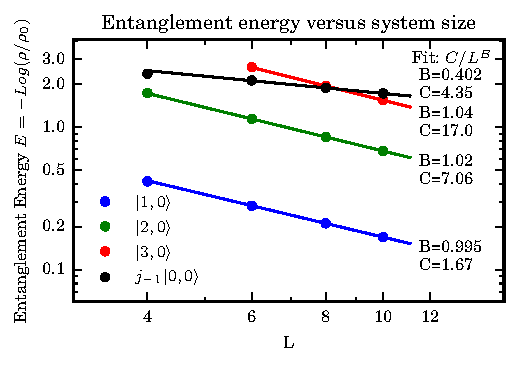
\includegraphics[width=2.5in]{{interpolatedboson/a10/plots/EntanglementEnergyScaling2.pdf}}
        %\caption{Power law fits for the lowest three states above the ground state at momentum zero and lowest two states at momentum 1 in Figure \ref{fig:sc-EEFinitesize}. The $1/L$ scaling is a signature of a gapless (entanglement) Hamiltonian. The labeling of the states $\ket{e, m}$ or $j_{-1} \ket{e, m}$ is explained in the CFT section below.}
        %\label{fig:sc-EEScaling}
        \end{figure}
        }
    \end{column}
\end{columns}
\end{frame}